
% this file is called up by thesis.tex
% content in this file will be fed into the main document

%: ----------------------- introduction file header -----------------------
\chapter{Inledning}

% the code below specifies where the figures are stored
\ifpdf
    \graphicspath{{1_introduction/figures/PNG/}{1_introduction/figures/PDF/}{1_introduction/figures/}}
\else
    \graphicspath{{1_introduction/figures/EPS/}{1_introduction/figures/}}
\fi

% ----------------------------------------------------------------------
%: ----------------------- introduction content ----------------------- 
% ----------------------------------------------------------------------
Många hållplatser i Malmö och andra städer är utsatta för vandalisering på olika möjliga sätt. Det handlar mest om hållplatser som är utanför stadens centrum eller utanför övervakningsområden. Det handlar om skadegörelser som kostar pengar, vilka kan utnyttjas till annat nödvändigt i staden. SAFE24, som kommer attt refereras till som gruppen härefter, sammanfattade sitt problem till att förhindra skadegörelser men även att hjälpa till att reda ut vem som ligger bakom en skadegörelse mot en busshållplats. 
\begin{figure}[h]

  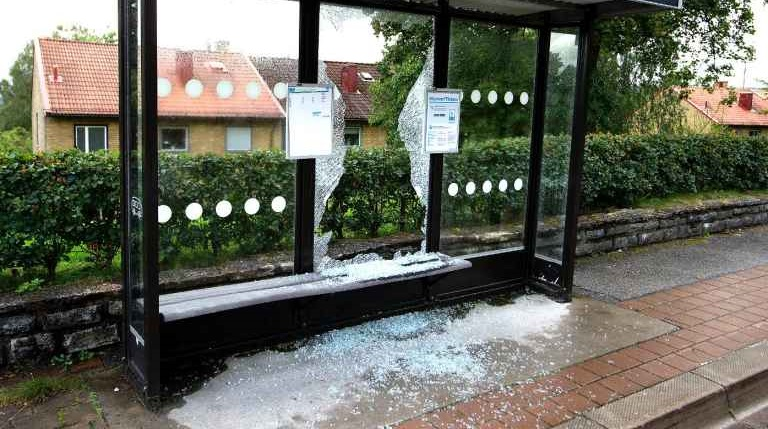
\includegraphics[width=\linewidth]{vandal.jpg}
  \caption{En vandaliserad hållplats i Borås.}
  \label{fig:vandal}
\end{figure}

%: ----------------------- HELP: latex document organisation
% the commands below help you to subdivide and organise your thesis
%    \chapter{}       = level 1, top level
%    \section{}       = level 2
%    \subsection{}    = level 3
%    \subsubsection{} = level 4
% note that everything after the percentage sign is hidden from output

\newglossaryentry{ANN}{name={ANN},
description={Artificial Neural Network, a generic name for different machine learning models that mimic how learning is done in nature.}}

%\section{put section name here} % section headings are printed smaller than chapter names
% intro



%\subsection{Name your subsection} % subsection headings are again smaller than section names
% lead
%Different organised systems have different energy currencies. The machines that enable us to do science like sizzling electricity but at a controlled voltage. Earth's living beings are no different, except that they have developed another preference. They thrive on various chemicals. 

% dextran, starch, glycogen
%Most organisms use polymers of glucose units for energy storage and differ only slightly in the way they link together monomers to sometimes gigantic macromolecules. Dextran of bacteria is made from long chains of $\alpha$-1,6-linked glucose units. 

%: ----------------------- HELP: special characters
% above you can see how special characters are coded; e.g. $\alpha$
% below are the most frequently used codes:
%$\alpha$  $\beta$  $\gamma$  $\delta$

%$^{chars to be superscripted}$  OR $^x$ (for a single character)
%$_{chars to be suberscripted}$  OR $_x$

%>  $>$  greater,  <  $<$  less
%≥  $\ge$  greater than or equal, ≤  $\ge$  lesser than or equal
%~  $\sim$  similar to

%$^{\circ}$C   ° as in degree C
%±  \pm     plus/minus sign

%$\AA$     produces  Å (Angstrom)




% dextran, starch, glycogen continued
%Starch of plants and glycogen of animals consists of $\alpha$-1,4-glycosidic glucose polymers \cite{lastname07}. See figure \ref{largepotato} for a comparison of glucose polymer structure and chemistry. 

%Two references can be placed separated by a comma \cite{lastname07,name06}.

%: ----------------------- HELP: references
% References can be links to figures, tables, sections, or references.
% For figures, tables, and text you define the target of the link with \label{XYZ}. Then you call cross-link with the command \ref{XYZ}, as above
% Citations are bound in a very similar way with \cite{XYZ}. You store your references in a BibTex file with a programme like BibDesk.





%\figuremacro{largepotato}{A common glucose polymers}{The figure shows starch granules in potato cells, taken from \href{http://molecularexpressions.com/micro/gallery/burgersnfries/burgersnfries4.html}{Molecular Expressions}.}

%: ----------------------- HELP: adding figures with macros
% This template provides a very convenient way to add figures with minimal code.
% \figuremacro{1}{2}{3}{4} calls up a series of commands formating your image.
% 1 = name of the file without extension; PNG, JPEG is ok; GIF doesn't work
% 2 = title of the figure AND the name of the label for cross-linking
% 3 = caption text for the figure

%: ----------------------- HELP: www links
% You can also see above how, www links are placed
% \href{http://www.something.net}{link text}

%\figuremacroW{largepotato}{Title}{Caption}{0.8}
% variation of the above macro with a width setting
% \figuremacroW{1}{2}{3}{4}
% 1-3 as above
% 4 = size relative to text width which is 1; use this to reduce figures




%Insulin stimulates the following processes:

%\begin{itemize}
%\item muscle and fat cells remove glucose from the blood,
%\item cells breakdown glucose via glycolysis and the citrate cycle, storing its energy in the form of ATP,
%\item liver and muscle store glucose as glycogen as a short-term energy reserve,
%\item adipose tissue stores glucose as fat for long-term energy reserve, and
%\item cells use glucose for protein synthesis.
%\end{itemize}

%: ----------------------- HELP: lists
% This is how you generate lists in LaTeX.
% If you replace {itemize} by {enumerate} you get a numbered list.


 


%: ----------------------- HELP: tables
% Directly coding tables in latex is tiresome. See below.
% I would recommend using a converter macro that allows you to make the table in Excel and convert them into latex code which you can then paste into your doc.
% This is the link: http://www.softpedia.com/get/Office-tools/Other-Office-Tools/Excel2Latex.shtml
% It's a Excel template file containing a macro for the conversion.

%\begin{table}[htdp]
%\centering
%\begin{tabular}{ccc} % ccc means 3 columns, all centered; alternatives are l, r

%{\bf Gene} & {\bf GeneID} & {\bf Length} \\ 
% & denotes the end of a cell/column, \\ changes to next table row
%\hline % draws a line under the column headers

%human latexin & 1234 & 14.9 kbps \\
%mouse latexin & 2345 & 10.1 kbps \\
%rat latexin   & 3456 & 9.6 kbps \\
% Watch out. Every line must have 3 columns = 2x &. 
% Otherwise you will get an error.

%\end{tabular}
%\caption[title of table]{\textbf{title of table} - Overview of latexin genes.}
% You only need to write the title twice if you don't want it to appear in bold in the list of tables.
%\label{latexin_genes} % label for cross-links with \ref{latexin_genes}
%\end{table}



% There you go. You already know the most important things.


% ----------------------------------------------------------------------



